  \documentclass[14pt, oneside]{book}
    \usepackage[margin=1in]{geometry} 
    \usepackage[brazilian]{babel}
    \usepackage{graphicx}
    \usepackage[utf8]{inputenc}
    \usepackage[T1]{fontenc}
    \usepackage{amsmath,amsthm,amssymb,amsfonts}
    \usepackage{enumitem}
    \usepackage{multicol}
    \usepackage{mathtools}
    \usepackage{titlesec}
    \usepackage{hyperref, color}
    \usepackage{float}
        \hypersetup{
            colorlinks=false, %set true if you want colored links
            linktoc=all,     %set to all if you want both sections and subsections linked
            linkcolor=blue,  %choose some color if you want links to stand out
        }
    \usepackage{listings}
    \titleformat{\chapter}[hang]{\bf\huge}{\thechapter}{2pc}{}
    \DeclarePairedDelimiter{\ceil}{\lceil}{\rceil}
    \date{\vspace{-5ex}}
    \lstset{language=Python}  
    \usepackage{pythonhighlight}
     
    \newcommand{\N}{\mathbb{N}}
    \newcommand{\Z}{\mathbb{Z}}
    \newcommand\tab[1][1cm]{\hspace*{#1}}
    \renewcommand{\qedsymbol}{$\blacksquare$}
     
    
\theoremstyle{definition}
    \newtheorem{problem}{Problema}
    \newtheorem{dica}{Dica}
    \newtheorem{gabarito}{Gabarito}
    \newtheorem{defn}{Definição}
    \newtheorem{teorema}{Teorema}
    
\begin{document}
    \pagenumbering{gobble}

    \begin{titlepage}
        \centering 
        
\includegraphics[scale = 0.8]{ufpe.png} \\
        \Large{\textbf{UNIVERSIDADE FEDERAL DE PERNAMBUCO}}\\
        \large{Departamento de Eletrônica e Sistemas}
        \vspace*{\stretch{2.0}}
   
        \Huge\textbf{ELETRÔNICA DIGITAL}\\
        \Large\textbf{DESPERTADOR/RELÓGIO}
   
        \vspace*{\stretch{2.0}}
        \vfill
        \Large{Arthur Santos Pimentel} \\
        \Large{Matheus Henrique Camilo de Araújo} \\
        \Large{Matheus Sobreira Farias} \\
        \Large{Pablo Godoy de Albuquerque}
        \\~\\
        \Large{Setembro, 2018}
    \end{titlepage}

\addtocontents{toc}{\protect\hypertarget{toc}{}}
\tableofcontents
\mainmatter
        \chapter[Motivação]{\hyperlink{toc}{Motivação}}
            \tab Um PLD, ou dispositivo lógico programável, é um componente eletrônico que é usado para construir circuitos digitais que são reprogramáveis. Um dispositivo lógico programável não tem uma função definida depois de fabricado, ao contrário de uma porta lógica, e tem que ser programado antes de poder ser usado. Existe uma grande variedade de dispositivos de lógica programável, dentre eles está o FPGA, que é um circuito integrado projetado para ser configurado por um consumidor ou projetista após a fabricação. Essa configuração é realizada por meio de uma linguagem de descrição de hardware. \\
	        \tab Linguagens de descrição de Hardware, ou HDLs, podem descrever o funcionamento do circuito, a sua concepção e organização, e ainda testá-lo para verificar seu funcionamento por meio de simulação. São padrões de expressões baseados em texto, da estrutura espacial, temporal e comportamental dos sistemas eletrônicos. Como outras linguagens de programação, HDLs incluem anotações explícitas para expressar a simultaneidade bem como sintaxe e semântica próprias. No entanto, em contraste com a maioria dos softwares de linguagem de programação, HDLs também incluem uma noção implícita de tempo, como um atributo primário de hardware. Uma das formas de fazer essa descrição é utilizando a linguagem de blocos. \\
	        \tab A eletrônica digital possibilitou a modernização de varios dispositivos, no presente trabalho, foi aplicado os conhecimentos de circuitos lógicos para a construção de um relógio/despertador digital.
           
            
        \chapter[Objetivos]{\hypertarget{obj}{}\hyperlink{toc}{Objetivos}}
             \tab Nesse projeto, foi utilizada a linguagem de blocos, com o auxílio do software \textit{Quartus Prime 17.1} e da placa \textit{FPGA DE2-155}, ambos da \textit{Altera}, com o intuito de criar um relógio/despertador, seguindo os seguintes critérios:
            \begin{itemize}
                \item A exibição do relógio ou despertador deve ser determinada por uma chave.
                \item O ajuste do relógio ou despertador deve ser determinada por uma segunda chave.
                \item Uma terceira chave deve ser utilizada para controlar o acionamento do despertador.
                \item Os botões da placa devem ser utilizados para efetuar o ajuste dos horários. Serão usados quatro botões para incrementar e decrementar as horas e os minutos.
                \item Serão utilizados quatro LEDs da placa para simular o acionamento do despertador.
            \end{itemize}
        \chapter[Implementação]{\hyperlink{toc}{Implementação}}
            \tab Para realizar a implementação do relógio/despertador, foi utilizado o software \textit{Quartus Prime 17.1}, que é um software cuja função é ser um ambiente de desenvolvimento para linguagens de descrição de hardware, sendo assim, a placa a qual foi descrita pelo projeto foi a \textit{Altera DE2-115}. Não foi utilizado ao longo do desenvolvimento nenhuma linguagem de descrição em código, justamente por ser um dos objetivos do projeto: implementar o relógio/despertador apenas com o uso de lógica digital e diagramas de bloco. \\
            \tab Uma vez no software \textit{Quartus}, para facilitar a construção do projeto, foi decidido separá-lo em \textbf{4} módulos de desenvolvimento, dessa forma o grupo como um todo conseguiria agir paralelamente, para que o tempo fosse melhor otimizado, são estes os módulos: \textbf{Up/Down Counter}, \textbf{Debounce}, \textbf{Seleção de Operação}, \textbf{Atrasador}.
            
            \section[Módulo Up/Down Counter]{\hyperlink{toc}{Módulo Up/Down Counter}}
                \tab Certamente o módulo mais importante de todo o projeto, o Up/Down Counter serve, como o próprio nome ja diz, como um contador. Para desenvolver o relógio/despertador, foi necessário a utilização de $6$ Up/Down Counter, pois foi preciso um contador para cada algarismo (unidades de segundo, dezenas de segundo, unidades de minuto, etc). Sendo os contadores de unidade com módulo $10$ (exceto o de unidade de hora, pois deve-se tomar cuidado por ser até $24$ horas) e os de dezena com módulo $6$ (exceto o de unidade de hora, pelo mesmo motivo). \\
                \begin{figure}[!h]
                    \centering
                    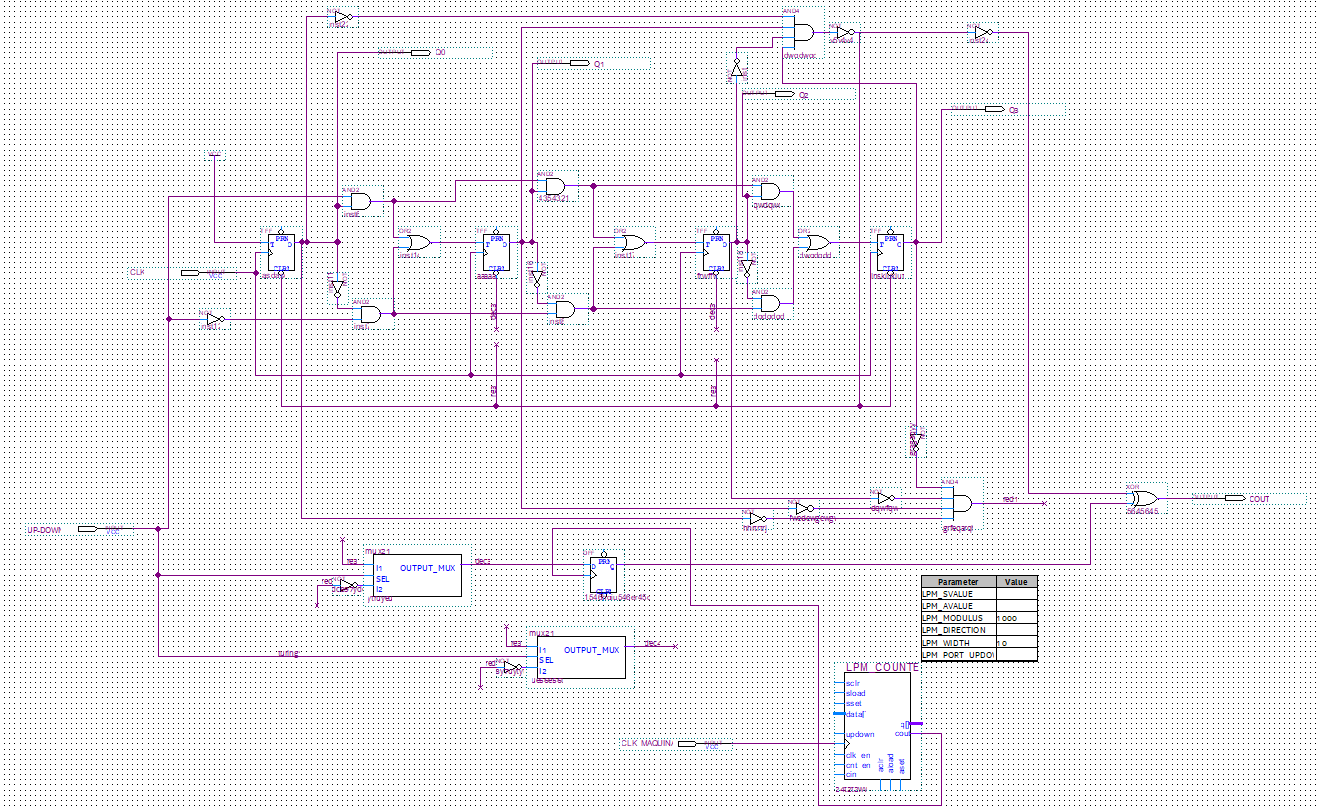
\includegraphics[scale = 0.5]{contadorupdownum.png}
                    \caption{Contador Up/Down de Unidade de Minuto}
                    \label{fig:unidadesegundo}
                \end{figure} \\
                \tab Como os contadores foram diferentes de módulo $2^n$, foi preciso estabelecer critérios de parada bem definidos, sendo no caso da Figura \ref{fig:unidadesegundo} os critérios de módulo $10$ para a chave selecionada em contador Up (\textbf{HIGH}), e um critério de parada para o valor $0$ para a chave selecionada em contador Down (\textbf{LOW}), sendo essa uma das grandes dificuldades da elaboração do projeto (será discutido melhor na seção de \hyperlink{ana}{Análise} do presente relatório.
                
            \section[Módulo Debounce]{\hyperlink{toc}{Módulo Debounce}}
                \tab O módulo Debounce surgiu como necessário a partir de um problema que ocorreu durante uma tentativa de teste do grupo. Ao testar o projeto em diferentes placas do laboratório, ocorreu de uma delas estar com o botão desgastado, de forma que, pressionando o botão rapidamente várias vezes, o ajuste de hora não incrementava/decrementava corretamente, e para corrigir isso, precisou ser implementado tal módulo. \\
                \tab A ideia por trás do Debounce gira em torno do ruído que é causado pelo botão ou alavanca, durante o momento do pressionar, conforme segue na Figura \ref{fig:debounce2}. \\
                \begin{figure}[!htb]
                    \centering
                    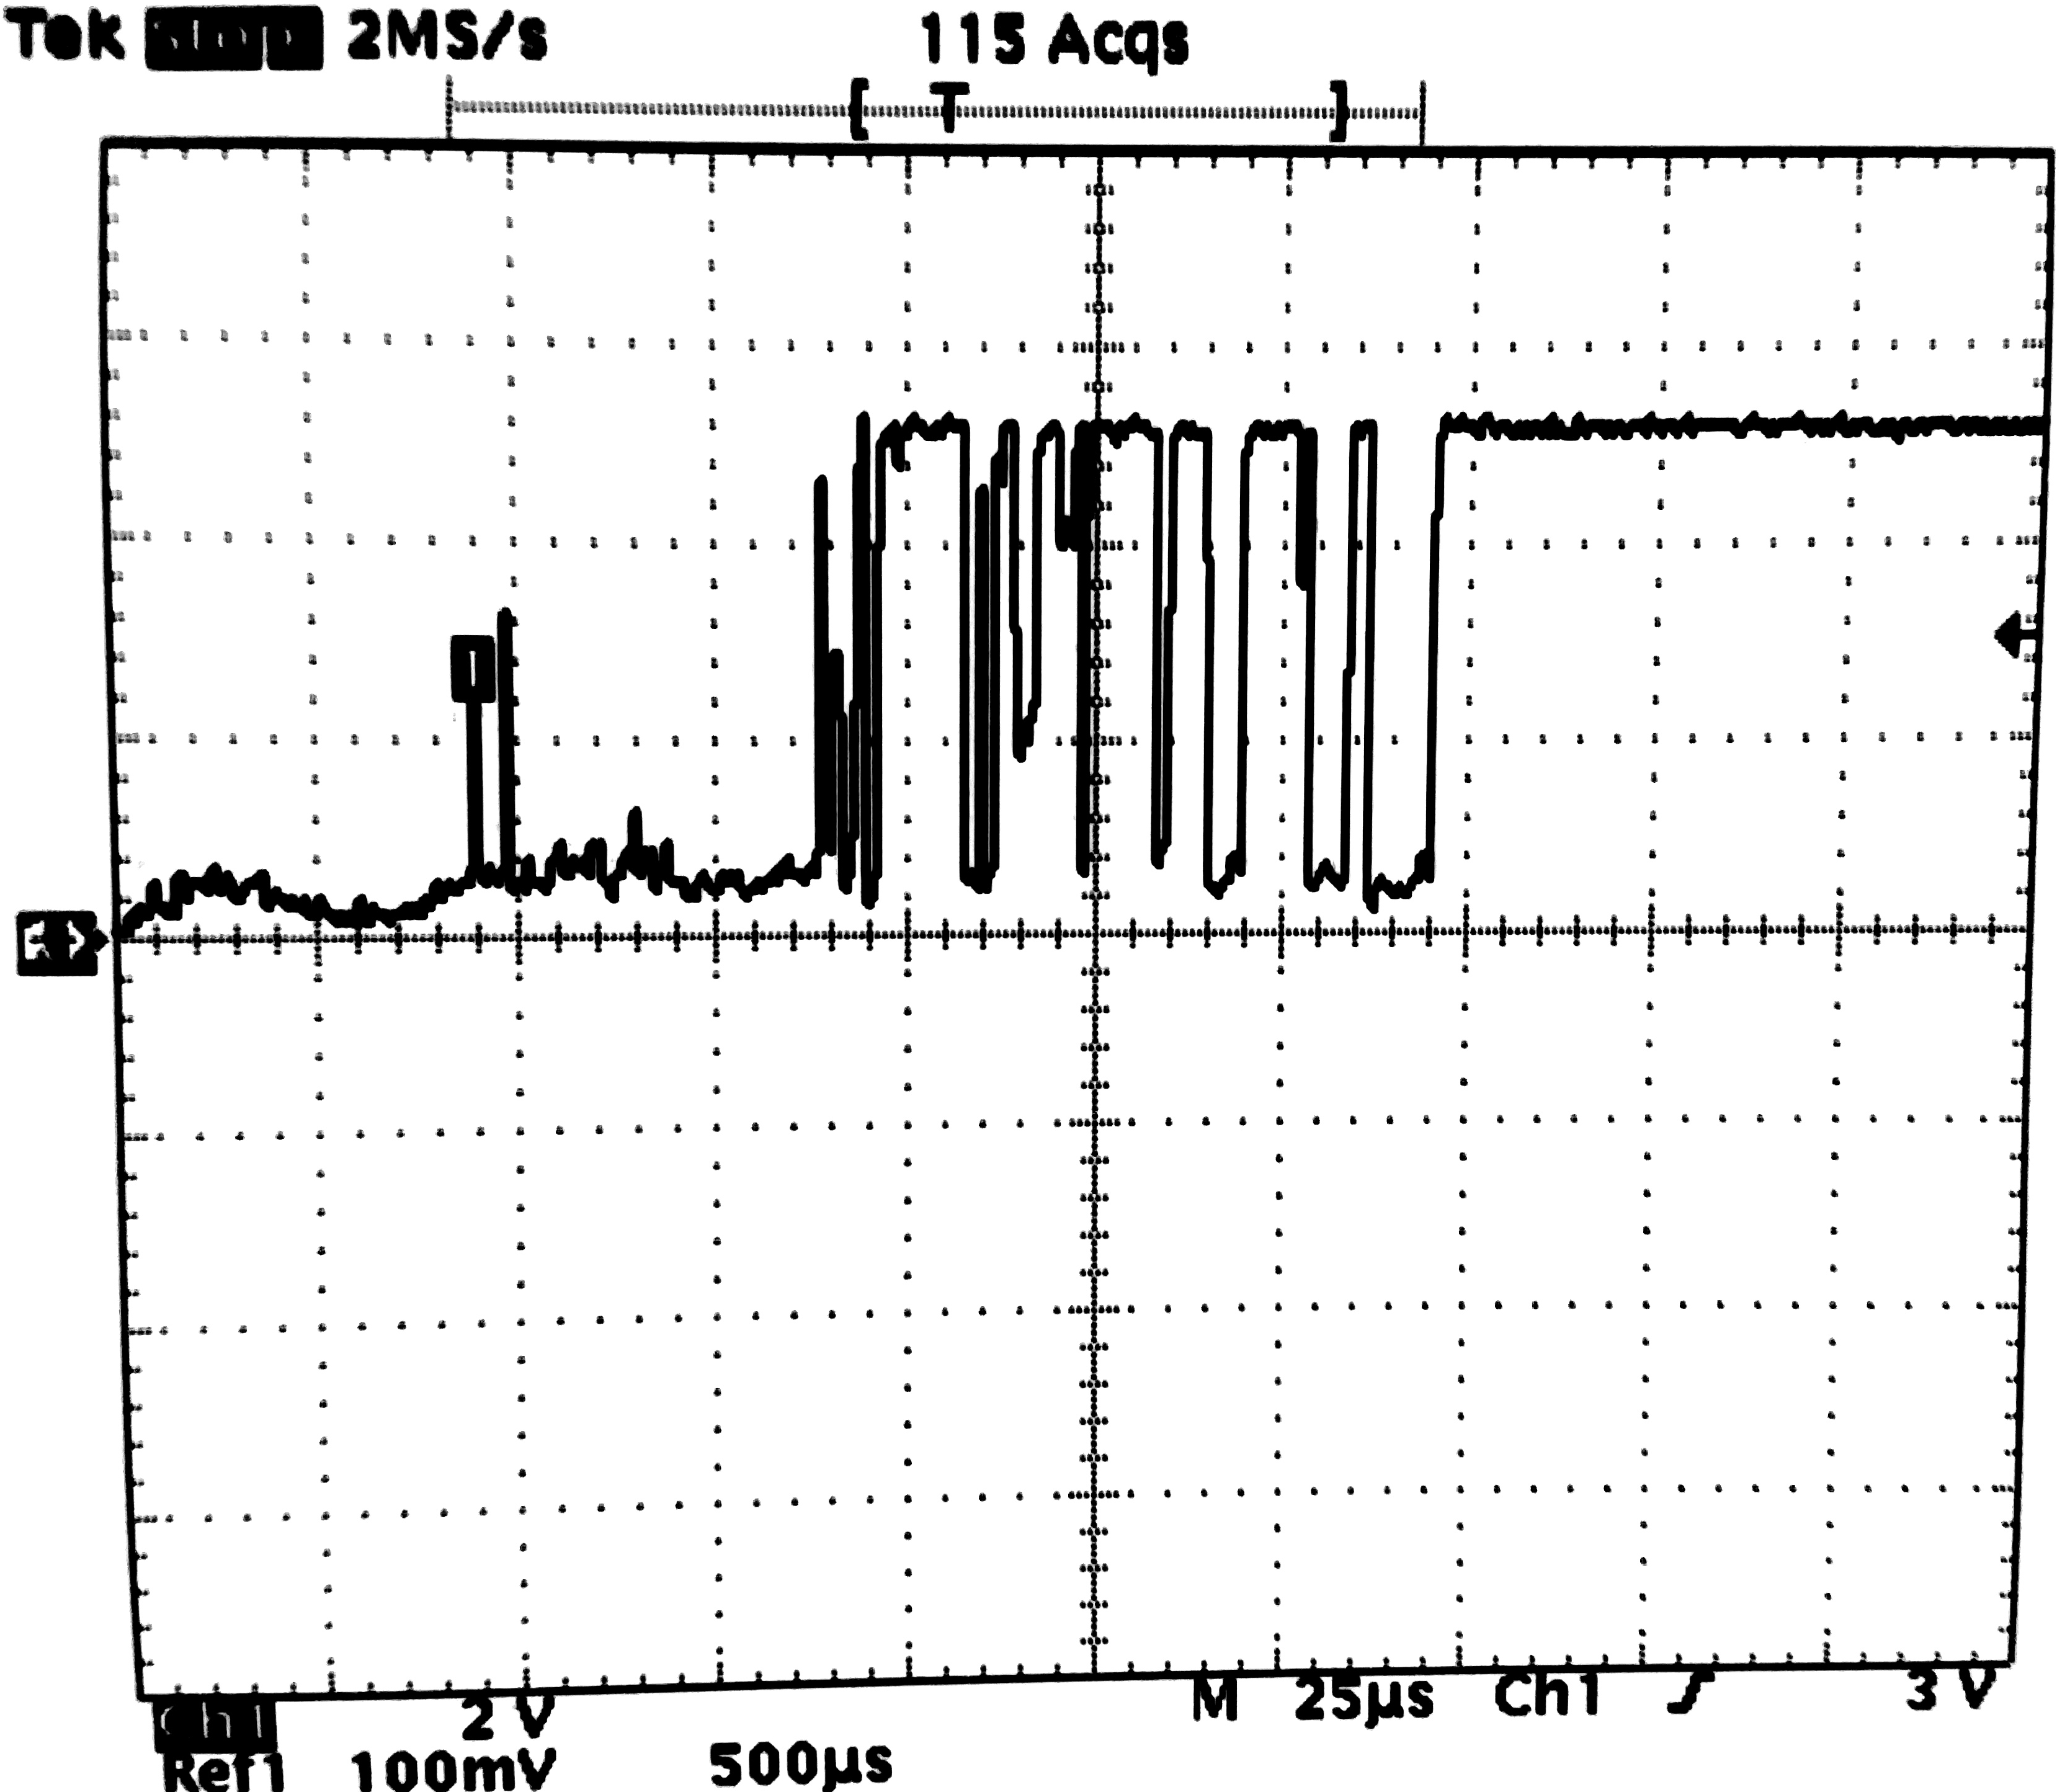
\includegraphics[scale=0.2]{debouncezao.png}
                    \caption{Ruído causado}
                    \label{fig:debounce2}
                \end{figure} \\
                \begin{figure}[!h]
                    \centering
                    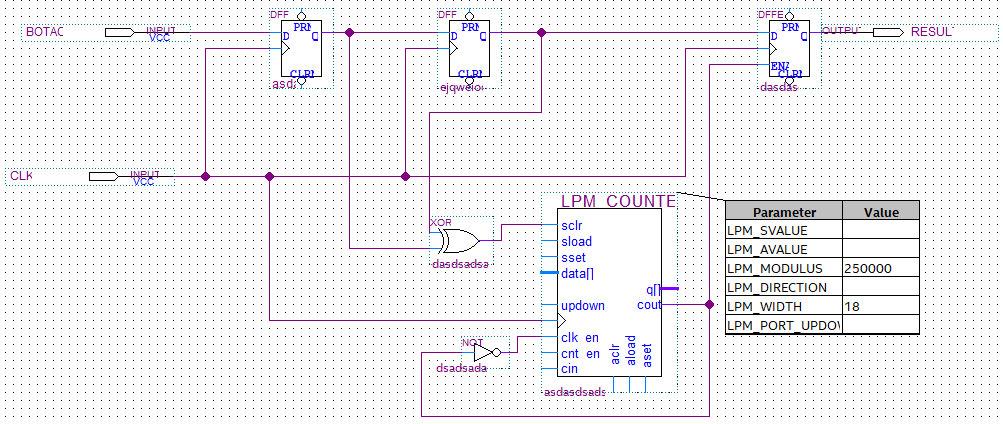
\includegraphics[scale=0.85]{debounce.png}
                    \caption{Módulo Debounce}
                    \label{fig:debounce}
                \end{figure} \\
                \tab Após a implementação do Debounce, o projeto foi testado em $3$ placas diferentes, de forma que funcionou de forma aceitável nas $3$ tendo como base o teste de pressionar rapidamente os botões.
                
            \section[Módulo Comparador]{\hyperlink{toc}{Módulo Comparador}}
                \tab O módulo Comparador foi idealizado para que pudesse ocorrer a comparação entre o horário atual e o horário definido para o despertador, de forma que se ocorrer a igualdade, quatro LEDs da placa são ativados em modo piscar durante o tempo de igualdade (os segundos são desconsiderados).
                \begin{figure}[!htb]
                    \centering
                    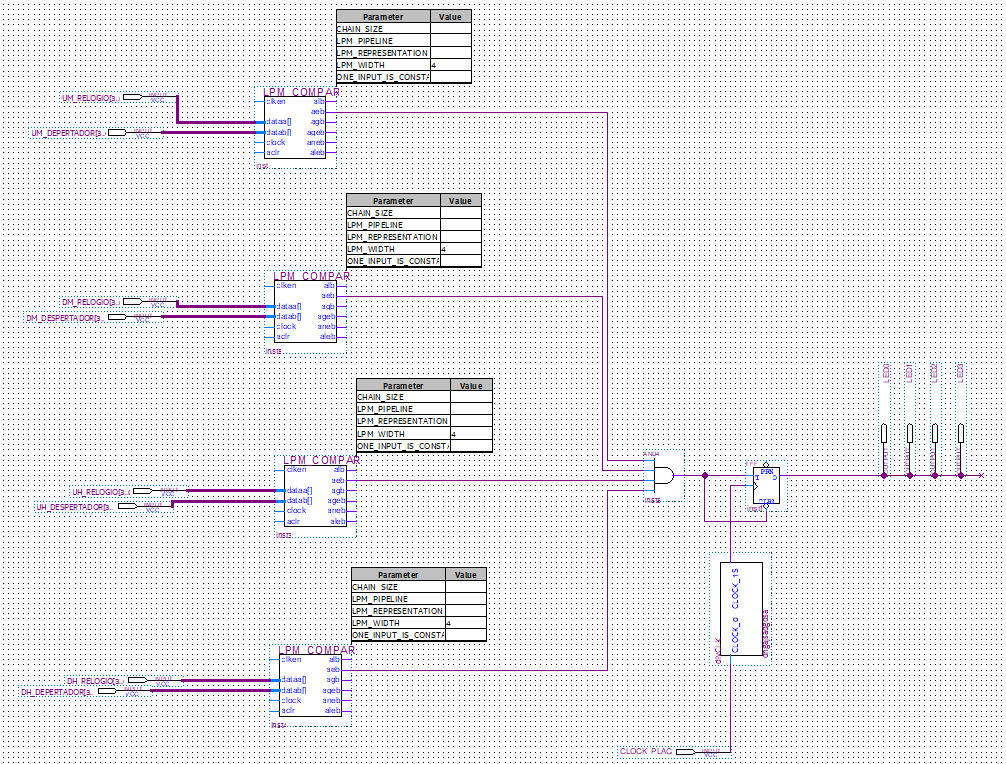
\includegraphics[scale = 0.6]{compare.png}
                    \caption{Comparador}
                    \label{fig:comparador}
                \end{figure} \\
                \begin{figure}[!htb]
                    \centering
                    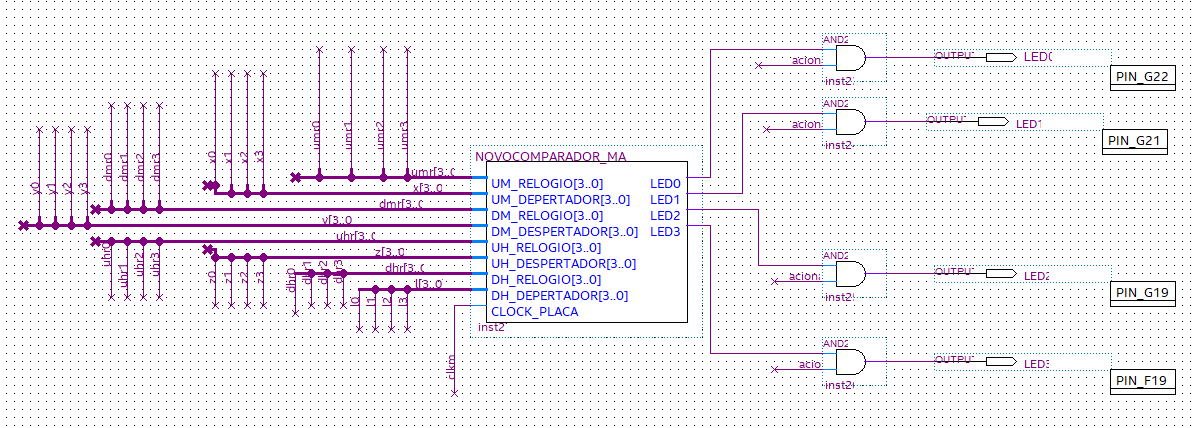
\includegraphics[scale = 0.6]{compare2.png}
                    \caption{Módulo Comparador}
                    \label{fig:comparador2}
                \end{figure} \\
            \section[Módulo de Seleção de Operação]{\hyperlink{toc}{Módulo de Seleção de Operação}}
                \tab Como o projeto possui dois modos de operação: Relógio ou Despertador, foi preciso elaborar um módulo que pudesse estabelecer a relação de escolha do que seria mostrado no display de 7 segmentos, por isso foi desenvolvido tal módulo, que envolve desde um mux para escolher entre o horário do relógio e do despertador em bits (mux 8:4) como também um decodificador para ler o valor do horário em binário e passar para o display como números de base decimal. \\
                \begin{figure}[!htb]
                    \centering
                    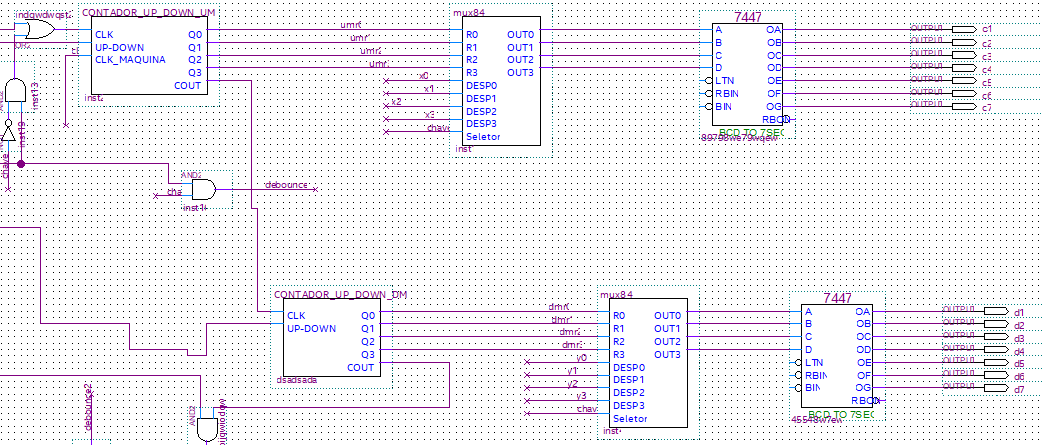
\includegraphics[scale=0.7]{relogio.png}
                    \caption{Seleção de Operação em Modo Relógio (minutos)}
                    \label{fig:seletor}
                \end{figure} \\
                \begin{figure}[!h]
                    \centering
                    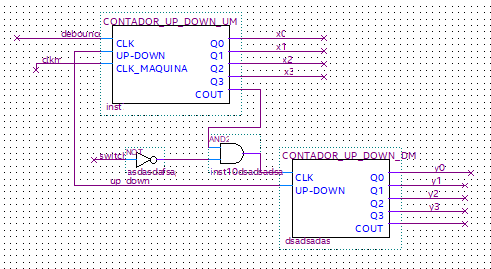
\includegraphics[scale=1.2]{despertador.png}
                    \caption{Seleção de Operação em Modo Despertador (minutos)}
                    \label{fig:seletor}
                \end{figure}
                
         \chapter[Manual de Operação]{\hyperlink{toc}{Manual de Operação}}
                \tab Esta seção é dedicada a esclarecer o funcionamento e organização da placa da \textit{Altera DE2-115}, bem como explicitar quais chaves, displays, LEDs e botões foram utilizados na implementação do relógio/despertador. \\
                \tab Observa-se um esquemático da placa na Figura \ref{manual}. Em que, \textbf{SW[17]} é a chave de ajuste ou exibição do que se encontra nos displays, \textbf{SW[16]} é a chave que determina a exibição do relógio ou despertador nos displays e \textbf{SW[15]} é a chave de acionamento do despertador, o LED da extrema direita é usado para indicar o modo de operação do despertador, enquanto o grupo de quatro LEDs indica igualdade entre despertador e relógio (toca alarme). Os quatro botões da placa são utilizados para realizar os incrementos e decrementos do relógio e despertador. O funcionamento desse botões são, respectivamente: incremento das horas, decremento das horas, incremento dos minutos e decremento dos minutos. \\
                \begin{figure}[!h]
                    \centering
                    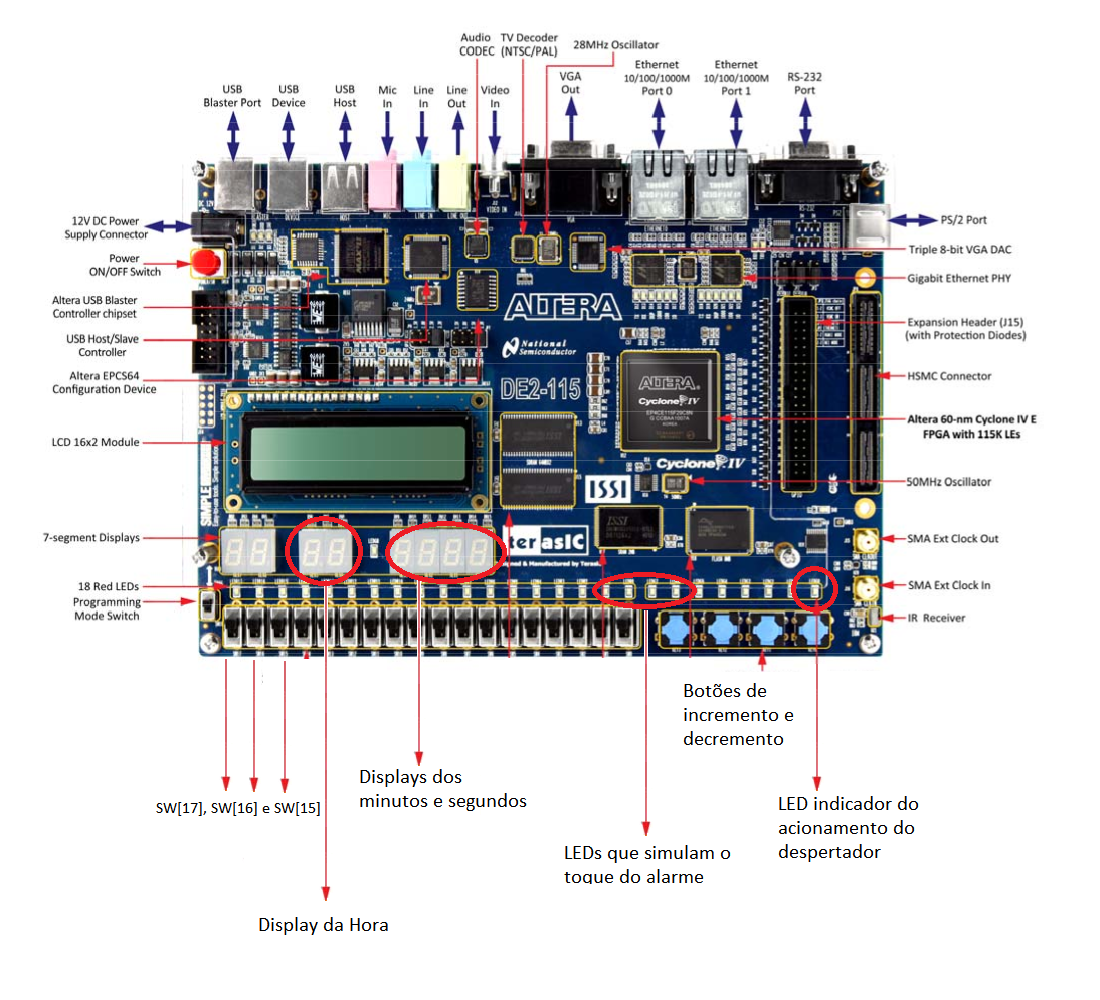
\includegraphics[scale=1]{manual.png}
                    \caption{Manual de Operação}
                    \label{manual}
                \end{figure}
                
            
        \chapter[Análise]{\hyperlink{toc}{Análise}} \hypertarget{ana}{}
            \tab No tocante aos problemas e dificudades encontradas no desenvolvimento do projeto cita-se as seguintes: \textbf{Atrasador}, \textbf{Mux 2:1}, \textbf{Ruidos}, \textbf{Contador} e \textbf{Botão}.
            
            \section[Atrasadores]{\hyperlink{toc}{Atrasadores}}
                \tab Ao longo do desenvolvimento do projeto, foi necessário a implementação de uma solução para o problema de sequenciamento de sinais: sinais desencadeados por uma mesma operação precisariam ser disparados em momentos diferentes, por isso foi usado um flip-flop tipo D, com um clock modificado, vide Figura \ref{fig:atrasador}.
                
                \begin{figure}[!h]
                    \centering
                    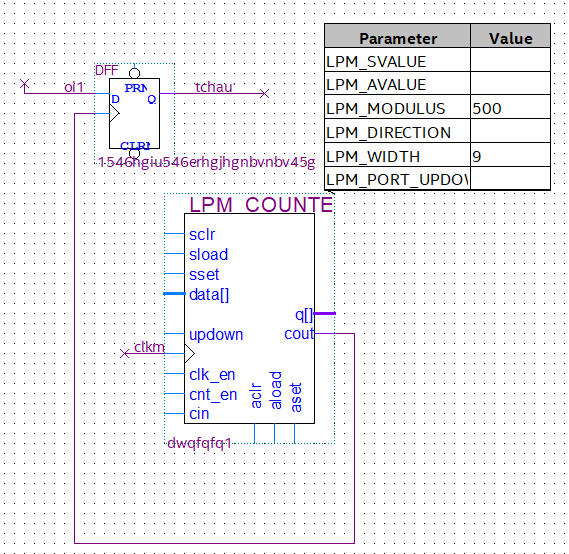
\includegraphics[scale=1]{atrasador.png}
                    \caption{Atrasador}
                    \label{fig:atrasador}
                \end{figure}
            
            \section[Mux 2:1]{\hyperlink{toc}{Mux 2:1}}
                \tab No desenvolvimento do projeto percebeu-se que o funcionamento do bloco do Mux 2:1 fornecido pelo \textit{Quartus} não era como esperado. Por isso, foi desenvolvido um bloco utilizando as portas lógicas AND, OR e NOT, que foi usado ao longo de todo o projeto.
                
                \begin{figure}[!h]
                    \centering
                    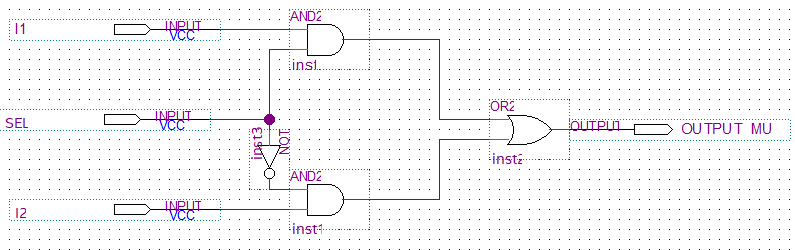
\includegraphics[scale=1]{mux21.png}
                    \caption{Mux 2:1}
                    \label{fig:mux21}
                \end{figure}
            
            \section[Ruídos]{\hyperlink{toc}{Ruídos}}
                \tab Ao realizar diferentes testes nas placas do laboratório, percebeu-se o não funcionamento adequado em algumas instâncias dos testes, que ocorriam de forma imprevisível. Assim, foi implementado o bloco Debounce com a finalidade de diminuir esses possíveis ruídos.
            
            \section[Contador]{\hyperlink{toc}{Contador}}
                \tab No desenvolvimento do contador foi encontrado o maior dos problemas do projeto. Este se trata da lógica necessária para realizar o decremento e incremento dos horários exibidos no display, onde a unidade deve ter resets diferentes, sendo módulo $4$ e $10$ para incremento e critério de reset $0$ para decremento e as dezenas tendo módulos $3$ e $6$ para incremento e reset $0$ para decremento, sendo as passagens de reset $0$ de decremento para os números $3$, $9$, $5$ ou $2$. Um exemplo é mostrado na Figura \ref{fig:decremento} \\
               \tab Foi utilizado uma lógica para resetar os flip-flops correspondentes a cada digito com a utilização de muxes seletores para resetar os flip-flops nos momentos específicos de transição, como bem mostrado na Figura \ref{fig:resets}.
                
                \begin{figure}[h!]
                    \centering
                    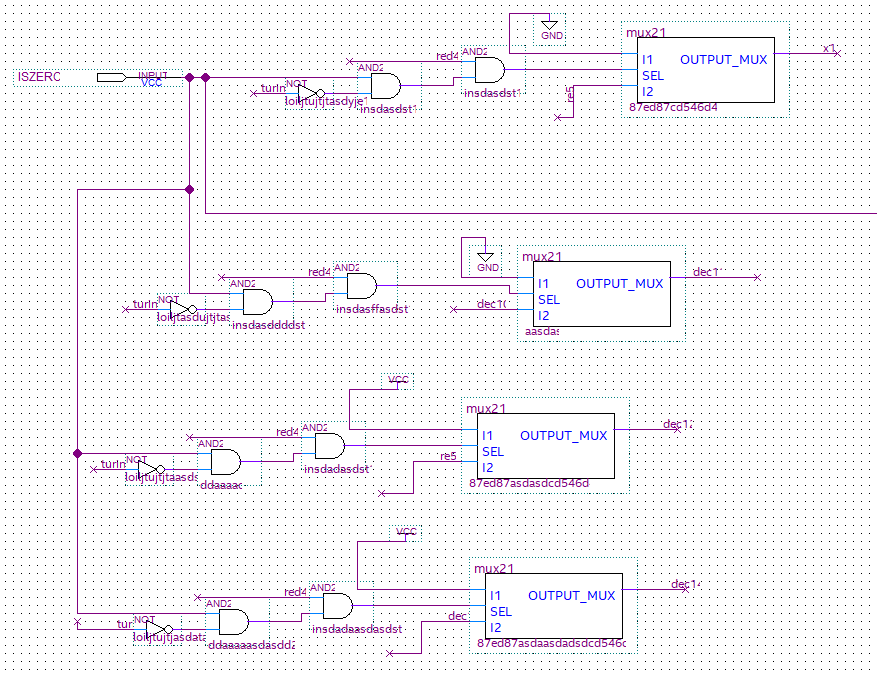
\includegraphics[scale=0.7]{decremento.png}
                    \caption{Condições de Reset}
                    \label{fig:decremento}
                \end{figure}
            
                \begin{figure}[!h]
                    \centering
                    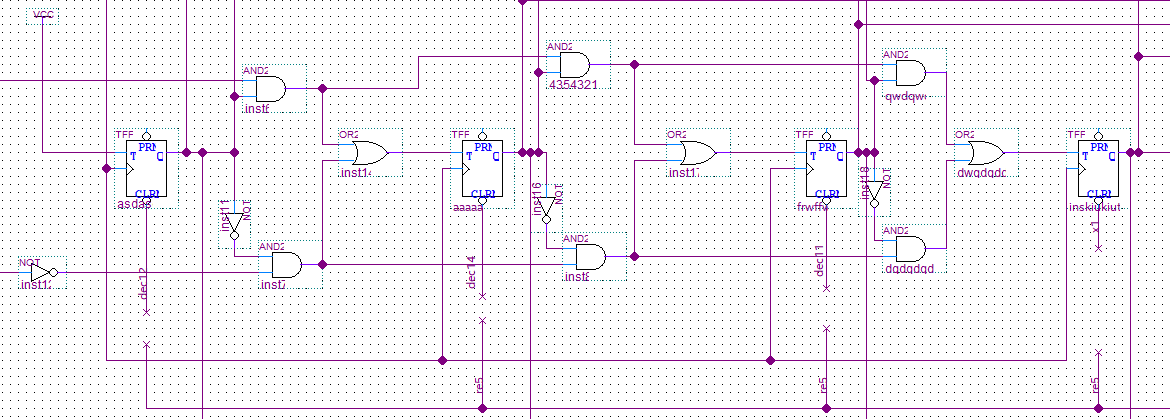
\includegraphics[scale=0.6]{resets.png}
                    \caption{Modificação nos Resets de Cada Dígito}
                    \label{fig:resets}
                \end{figure}
                
            \section[Botão]{\hyperlink{toc}{Botão}}
                \tab Como o contador Up/Down depende de ter a informação se o botão pressionado é de incremento ou de decremento, foi preciso elaborar alguma forma de separar tal informação, visto que naturalmente os botões marcam 1 (\textbf{HIGH}) quando não estão pressionados e 0 (\textbf{LOW}) quando estão pressionados, sendo assim não se diferenciam. \\
                \tab Para isso, foi criado uma lógica de escolha através do flip-flop J-K, de tal forma que os botões entram barrados nas entradas J e K, e a saída $1$ (\textbf{HIGH}) representa que o botão pressionado foi o de incremento, enquanto a saída $0$ (\textbf{LOW}) representa que o botão pressionado foi o de decremento, conforme mostrado na Figura \ref{fig:botoes}
                
                \begin{figure}[!h]
                    \centering
                    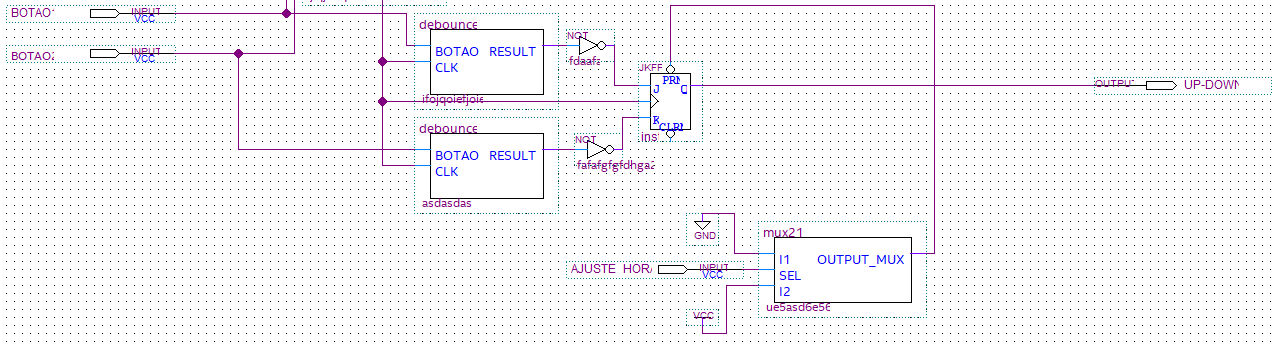
\includegraphics[scale=0.5]{botoes.png}
                    \caption{Lógica de Up/Down dos Botões}
                    \label{fig:botoes}
                \end{figure}
            
         \chapter[Limitações]{\hyperlink{toc}{Limitações}}
            \tab Um grande problema que foi enfrentado está relacionado diretamente ao fato da forma de escolha dos botões terem sido a partir de um flip-flop J-K. Sabe-se que tal flip-flop memoriza o valor da saída, de tal forma que a saída do flip-flop é um sinal constante e de valor 1 (\textbf{HIGH}) se o botão pressionado for de incremento, e um sinal constante de valor 0 (\textbf{LOW}) se o botão pressionado for de decremento, e por este fato, a saída elimina a característica de \textbf{pulso} que o botão tem, passando a atuar similarmente a uma alavanca, na Figura \ref{fig:segura} pode-se ver no canto superior a lógica de um botão retornar o valor 1 (\textbf{HIGH}) apenas quando pressionado, e quando não pressionado, retornar o valor 0 (\textbf{LOW}), e no canto inferior tem-se a ideia da saída implementada do flip flop J-K, onde o flip flop retorna o valor 0 (\textbf{LOW}) até o instante em que o botão é pressionado, a partir dai, o valor retornado é 1 (\textbf{HIGH}), mesmo que o botão não esteja mais sendo pressionado. \\
            \begin{figure}[!h]
                    \centering
                    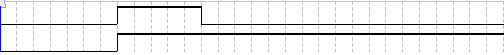
\includegraphics[scale=1.3]{segura.png}
                    \caption{Botão vs Flip-Flop J-K}
                    \label{fig:segura}
                \end{figure} \\
            \tab Diante disso, surgiram 3 glitches no projeto:
            \begin{itemize}
                \item Se o J-K que representa a hora ou o minuto estiver em $1$ (\textbf{HIGH}) e o valor da unidade de hora ou de minuto for $0$, ao pressionar o botão de decrementar, a unidade irá para $9$, enquanto a dezena permanecerá fixa
                \item Se o J-K que representa a hora ou o minuto estiver em $0$ (\textbf{LOW}) e o valor da unidade de hora ou de minuto for $0$, ao pressionar o botão de incrementar, a unidade e a dezena serão incrementadas de $1$.
                \item Se o J-K que representa a hora ou o minuto estiver em $0$ (\textbf{LOW}) e a alavanca de seleção de modo for selecionada para modo ajuste, a dezena de hora ou minuto será acrescentada de $1$.
            \end{itemize} \\
            \tab Como os glitches são bastante específicos e não contribuem significativamente para o funcionamento do relógio/despertador, não foi considerado um erro tão grosseiro pelos integrantes do grupo.
            
        \chapter[Conclusão]{\hyperlink{toc}{Conclusão}}
            \tab Com a exceção das limitações anteriormente mencionadas, o projeto desenvolvido foi bem sucedido. Uma vez que os principais critérios, abordados nos \hyperlink{obj}{Objetivos}, foram cumpridos. \\
            \tab Observa-se o bom funcionamento da operação do modo relógio, quando se trata do sincronismo dos contadores usados para as unidades e dezenas dos segundos, minutos e horas. Bem como o modo ajuste, que permite incrementar e decrementar as horas e minutos do relógio e do despertador. Além disso, realizou-se com êxito o modo comparador para o relógio e despertador, o qual aciona quatro LEDs piscantes da placa quando é verificado que o horário indicado pelo relógio e despertador são iguais. \\
            \tab Diante do apresentado, durante o desenvolvimento do projeto, percebeu-se que a implementação de um relógio com despertador usando a linguagem de blocos mostrou-se desafiadora, visto que não é possível usar estruturas condicionais e de repetição. Ademais, vale ressaltar que a estrutura escolhida para o desenvolvimento do projeto visou a criação de um relógio no modelo mais fiel à máquina, de tal forma que a ideia principal baseou-se em dividir clocks, e não em uma calculadora com memória, somando e subtraindo bits.
                    
        
        
\end{document}